\section{实验3:AI基于中性广告生成高低水平个性化广告的能力}

实验2验证了AI在不同产品类型的中性广告基础上生成个性化广告的能力,结果表明AI能够在享乐型与实用型产品中提取相应的个性化策略,并针对不同人格特质生成有效的个性化广告。然而,实验2仅关注了针对高水平人格特质(如高开放性、高尽责性)的个性化生成,未涉及低水平人格特质的定制设计。在实际应用中,广告不仅需要满足高水平特质个体的需求,还可能需要针对低水平特质个体进行设计,以覆盖更广泛的受众群体。

另一方面,针对高低水平人格特质的个性化效果,在现有文献中并未得到一致的验证。\citet{matz2017psychological}在其大样本实践研究中仅检验了开放性和外倾性分别针对高低水平设计的有效性,未涉及所有人格特质。而在\citet{matz2024potential}基于GPT生成个性化广告的研究中,不同实验间的结果也存在不一致性:部分实验中,针对高低水平设计的个性化广告在开放性、尽责性和外倾性维度上效果显著,但宜人性未能得到稳定的结果。同时,不同因变量(如广告效果与支付意愿)的测量中,高低水平的个性化效果差异也不稳定,尤其是外倾性维度,在某些实验中表现显著,而在另一些实验中则未表现出显著性。

基于上述研究的不一致性,以及实验2未覆盖低水平人格特质的局限,实验3旨在进一步探讨AI在双重人格水平(高水平与低水平)情境下生成个性化广告的能力,并验证高低水平特质的个性化效果是否存在显著差异。这不仅有助于完善现有文献中的空白,也为AI生成的个性化广告在更复杂场景中的应用提供可靠依据。但在本实验中我们不会涉及神经质特质的个性化设计,因为神经质的特性较为独特,其在低水平端的匹配信息(即针对情绪稳定性的设计)往往对高水平和低水平个体均具有吸引力 \citep{matz2016personality},因此难以实现真正针对高低水平的有效区分。


\subsection{方法}


\textbf{(1)被试}

通过见数平台发布实验,356名参与者自愿参加这项研究。36名参与者由于注意检查测试未通过被剔除,剩余\textbf{320名有效参与者}(年龄范围= 18-59岁;\textit{M}=26.06岁;\textit{SD}=7.90;女性200名)。参与任务的每名参与者获得1元人民币作为报酬。注意力检测包含两部分,分别嵌入在因变量测量和人格问卷中,以明确指令题形式呈现(如“请选2”)。参与者需在两道注意力检测题中均作答正确,方可被纳入有效数据样本。每名被试会随机分配到四个特质(开放性、尽责性、外倾性、宜人性)的条件之一,最终每个特质条件均有约80名被试参与。


\textbf{(2)实验材料:广告设计}

本实验共设计\textbf{2(水平:高/低)* 4(特质:开放性、尽责性、外倾性、宜人性)共8则个性化广告}。这些广告均基于一则来自微博平台的热门新款手机中性广告,通过GPT的文本生成与调整功能进行个性化设计。中性广告从当前热门的手机品牌官方广告中筛选而来,考虑到本实验的测量方式旨在比较不同的广告效果,因此品牌效应在比较中被抵消。同时,保留品牌信息能够增强广告的真实性和实验情境的生态效度,因此在本实验中未移除广告中的品牌信息。原广告示例如图\ref{fig:Study1-substudy3-originalAd}所示。针对每个特质与水平的组合,我们使用了GPT生成个性化广告文案(详见附录)。生成过程基于一套结构化的提示语(prompt),提示语(详见附录)包含以下关键要素:任务目标,原始广告文案,调整优化的要求,策略说明。为验证个性化广告的有效性,本研究在正式实验前通过见数平台发布了预实验,共有90名参与者自愿参加,并获得1元人民币作为报酬。每名参与者需对8则广告的目标消费者群体进行选择,具体任务为从2(水平)*5(特质)中选择出最匹配的目标消费者。预实验结果显示,大多数参与者能够正确识别出各广告的目标消费者特质,这表明GPT生成的个性化广告在针对特定人格特质的目标消费者设计上具有有效性。

\begin{figure}[H]
    \centering
    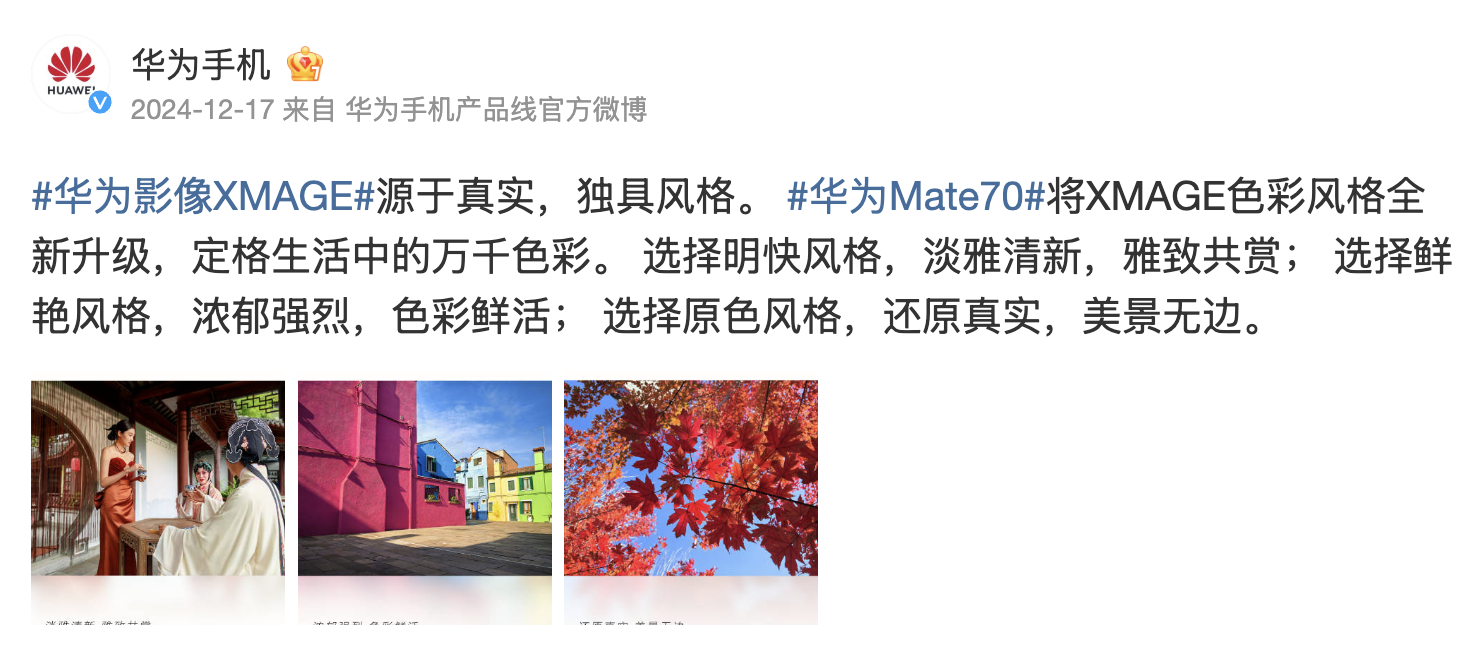
\includegraphics[width=.8\linewidth]{Image/Study1-exp3-original ad.png}
    \caption{\label{fig:Study1-substudy3-originalAd}微博提取广告示意图}
\end{figure}



\textbf{(3)问卷测量}
\label{study1-substudy3-measures}

a. 大五人格量表
本实验从\citet{john1991big}编制的44道题目大五人格量表(BFI-44)中筛选出与目标特质相关的题目。参与者根据其被分配到的人格特质类别完成相应题目。每个题项采用1-5点李克特量表,1分表示“完全不符合”,5分表示“完全符合”。

b. 广告说服效果
实验中,高水平与低水平的个性化广告以并排形式随机呈现,分别标记为广告A和广告B。参与者需对两则广告的偏好进行评分,评分采用11点双极量表(如图\ref{fig:Study1-exp3-rating}),分值范围从“更倾向于广告A”到“更倾向于广告B”。为避免顺序效应,广告A/B呈现顺序随机化。为便于结果解读,在数据统计时将评分结果进行转换,使得分数越高表示参与者对高水平的个性化广告的偏好越强,分数越低表示参与者对低水平的个性化广告的偏好越强。

具体测量题项与实验2保持一致,共包括五个题项,分别评估参与者对广告和产品的态度及其购买意图。广告说服效果的总评分为五个题项得分的平均值。

c. 关键词选择
在广告说服效果评分完成后,参与者还需从每则广告中选出最吸引他们的Top3关键词。这些关键词用于后续分析,以进一步探讨个性化广告的有效性。例如,通过比较高水平与低水平广告中被选出的关键词,评估不同人格特质的参与者是否更倾向于关注与其特质匹配的广告要素。

\begin{figure}[H]
    \centering
    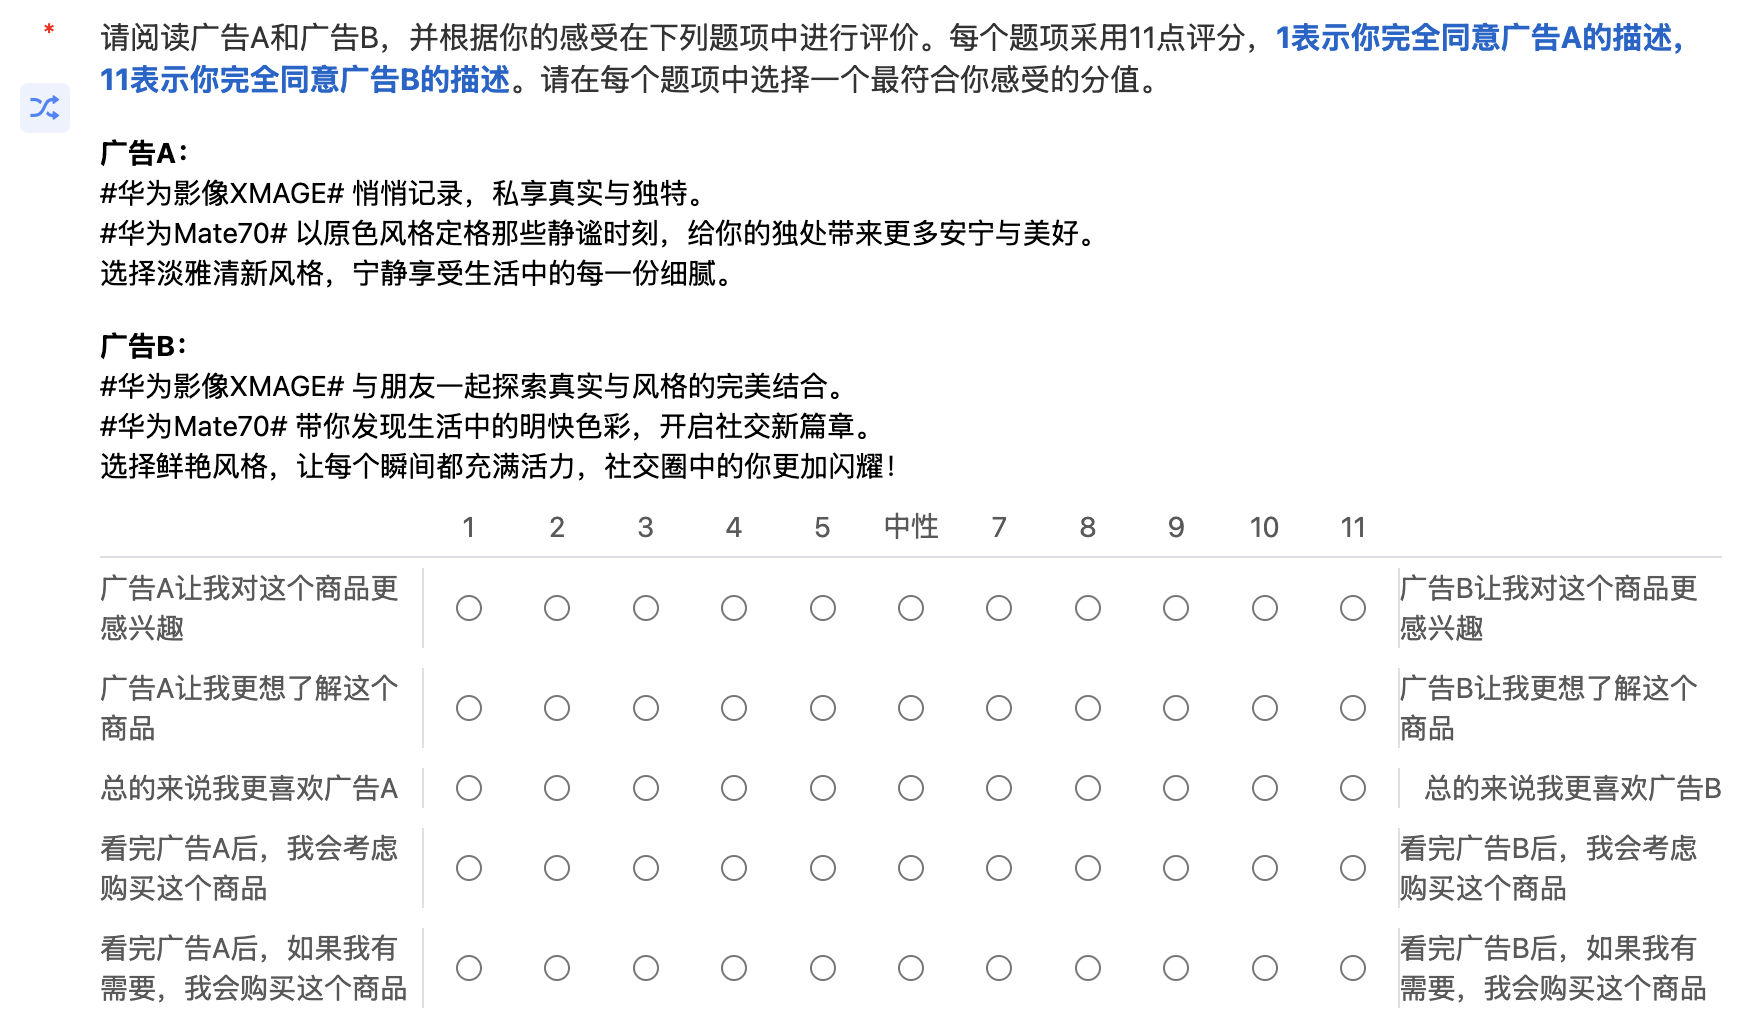
\includegraphics[width=.8\linewidth]{Image/Study1-exp3-rating.png}
    \caption{\label{fig:Study1-exp3-rating}实验评分示意}
\end{figure}


\subsection{实验流程}
本实验流程分为两个部分。第一部分,参与者依次阅读每组广告,其中每组广告包含高水平与低水平的个性化广告(例如,针对高外倾性和低外倾性设计的广告),并对每组广告的相对说服效果进行评分。第二部分,参与者完成与人格测试相关的问卷,随后填写包括年龄、性别等在内的人口统计学信息。

\subsection{结果}
我们分别对每个特质的结果进行了回归分析。回归模型的自变量为参与者对应人格特质的得分(尽责性、开放性、外倾性、宜人性),因变量为广告的说服效果。由于评分为二极分布,我们对数据进行了转换,使得得分越高表示相较于低水平个性化广告,参与者对高水平个性化广告的偏好越强。在这一模型中,如果存在匹配效应(即高水平特质的参与者更偏好针对高水平设计的个性化广告,而低水平特质的参与者更偏好针对低水平设计的个性化广告),则回归系数应为正且显著。

结果如图\ref{fig:Study1-exp3-result}所示,展示了针对四种人格特质设计的广告组的标准化效应及其95\%置信区间。结果表明,开放性(\textit{$\beta$} = 1.729,\textit{p} < 0.01)、外倾性(\textit{$\beta$} = 2.451,\textit{p} < 0.001)和宜人性(\textit{$\beta$} = 1.864,\textit{p} < 0.05)的得分显著预测了参与者对相应特质个性化广告的偏好。这意味着,在这些特质维度上,水平较高的参与者更偏好针对高水平设计的广告,水平较低的参与者则更偏好针对低水平设计的广告。然而,对于尽责性(\textit{$\beta$} = 0.101,\textit{p} = 0.898)维度,未观察到类似的匹配效应,表明无论是高尽责还是低尽责的参与者,在广告偏好上表现出相似的趋势。

\begin{figure}[H]
    \centering
    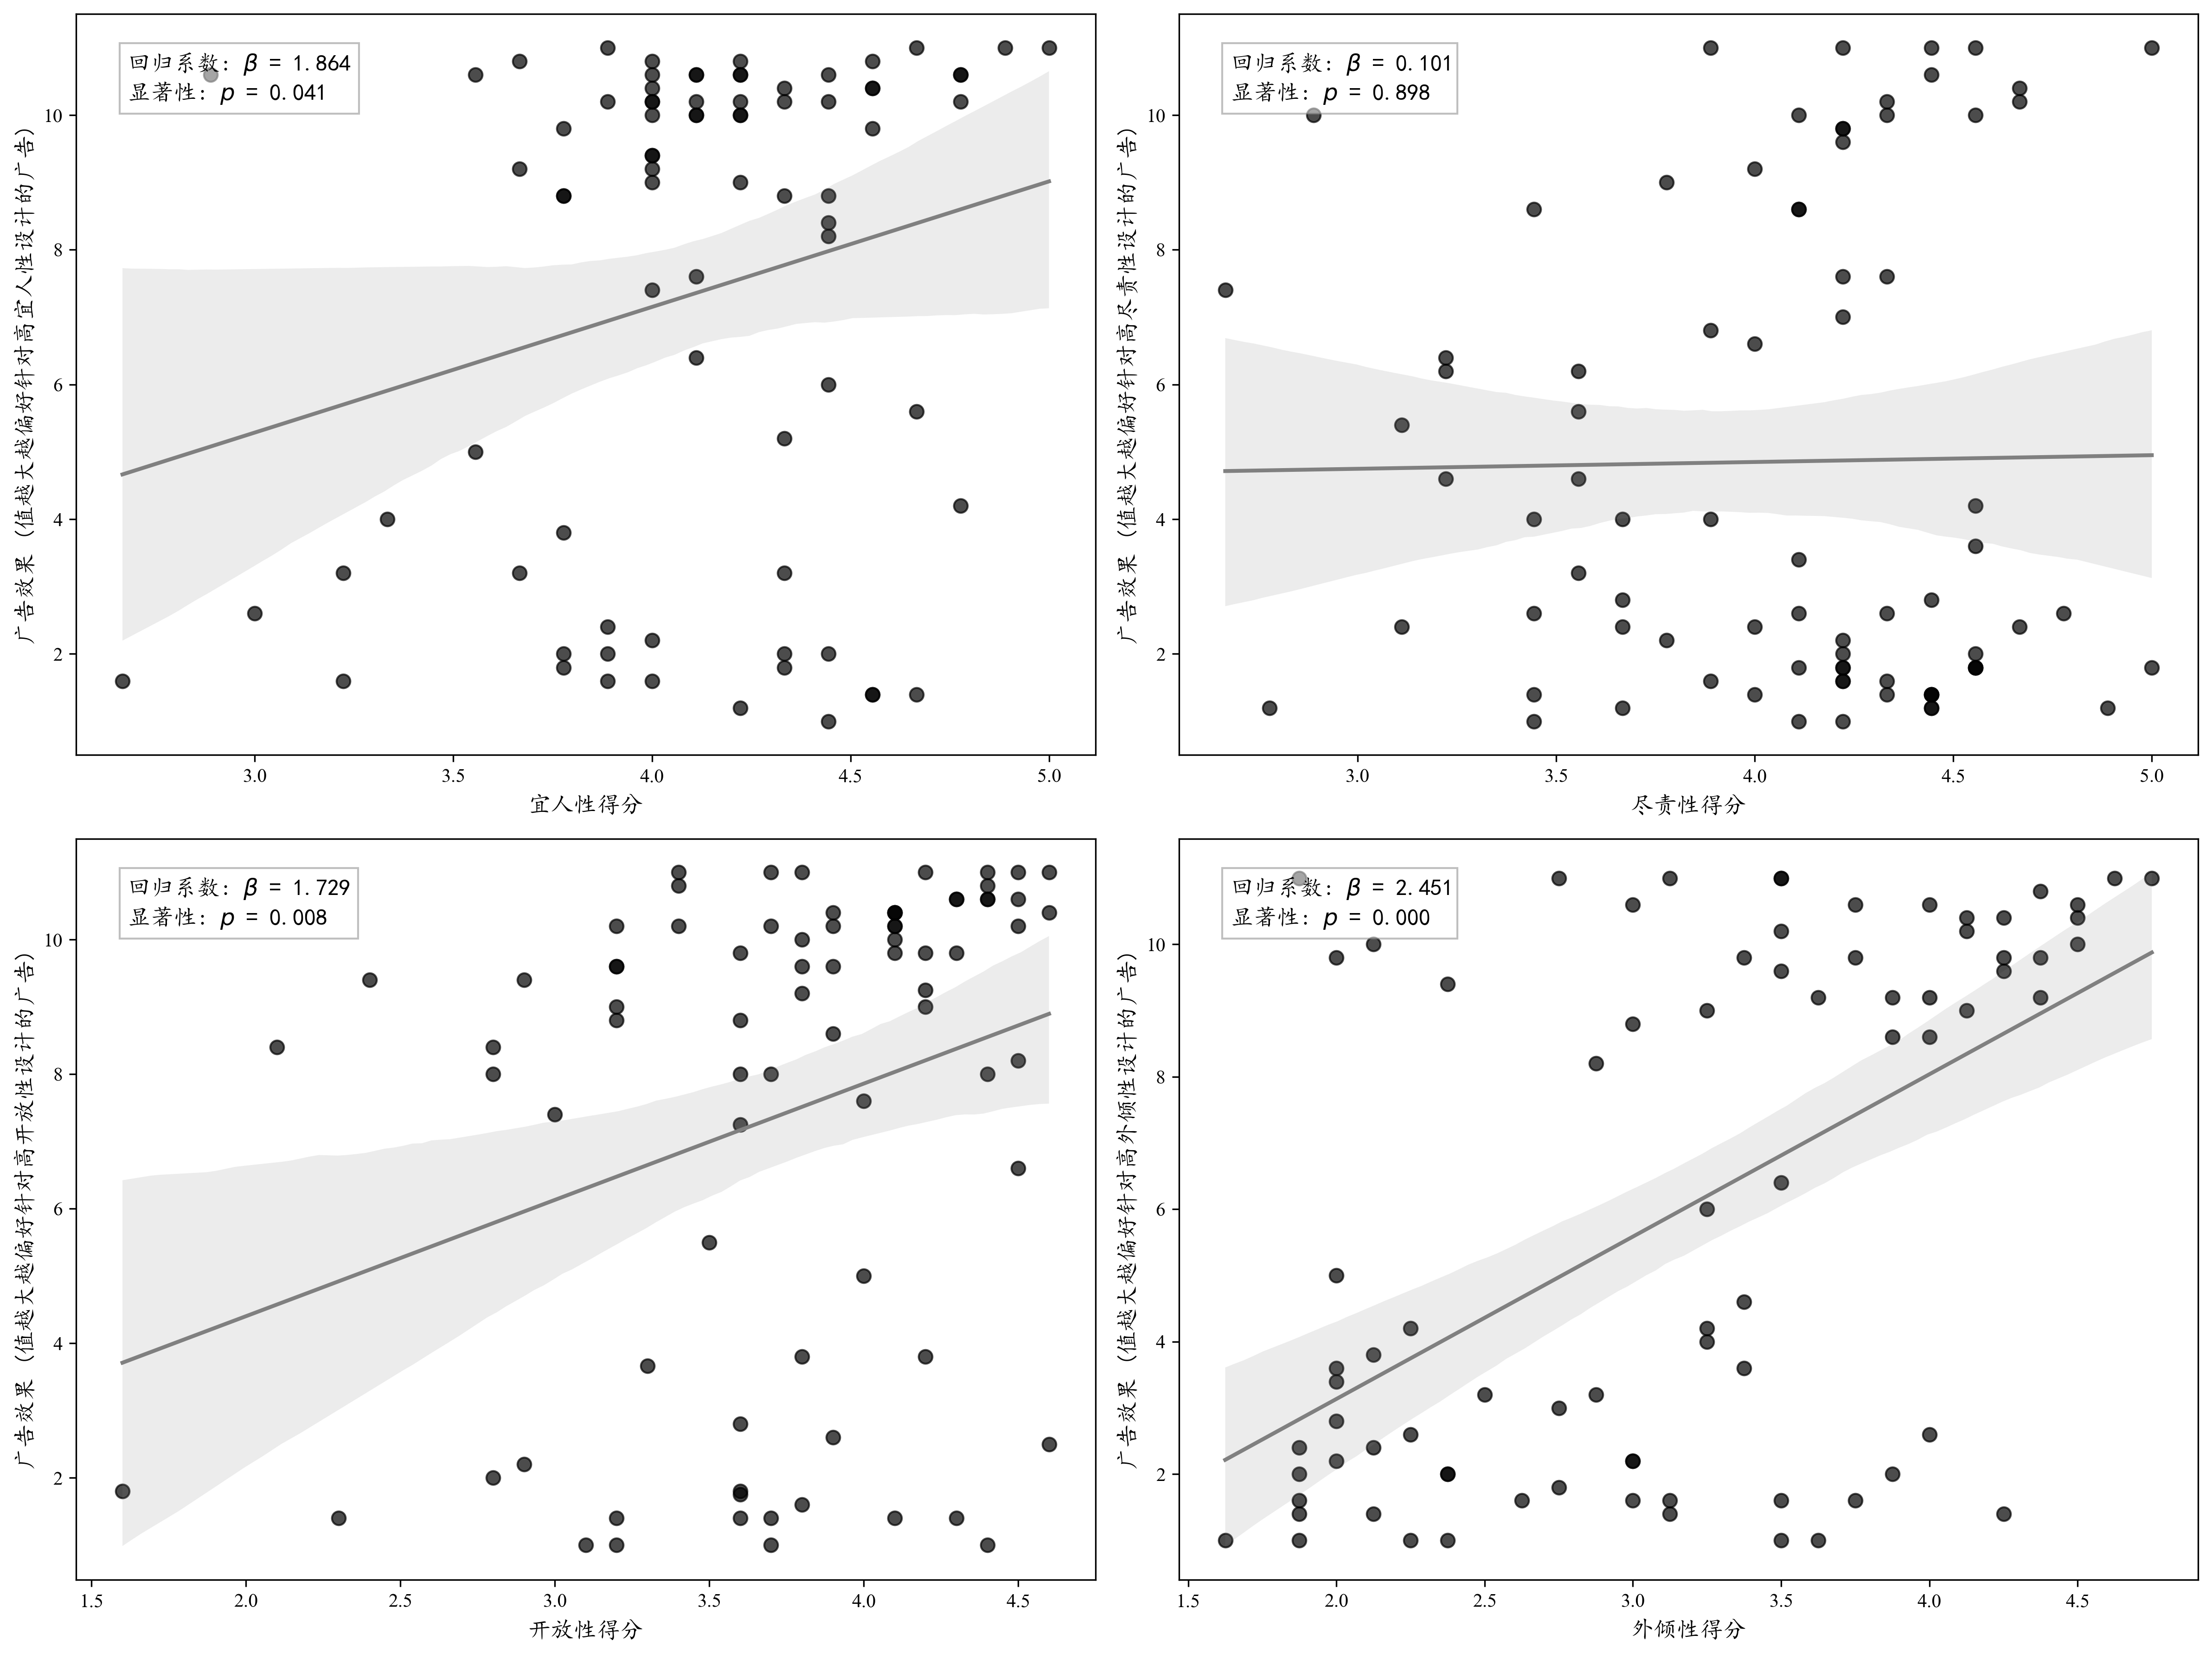
\includegraphics[width=1.0\linewidth]{Image/Study1-exp3-result.png}
    \caption{\label{fig:Study1-exp3-result}四个人格特质对相应广告效果评分的影响(含95\%置信区间)}
\end{figure}

为进一步探讨参与者偏好个性化广告的原因,我们将参与者按人格水平的中值划分为高水平组和低水平组,并筛选出他们在偏好广告中选择的Top 3关键词(根据广告说服效果评分,得分≥6表示更偏好针对高水平设计的广告,<6表示更偏好针对低水平设计的广告),对这些关键词进行词频统计和分析。这种方法能够揭示不同人格水平的个体在广告偏好上的差异,从而帮助解释个性化广告效果的背后机制。

针对回归分析中个性化效果显著的宜人性(表\ref{tab:agreeableness_neutrl_preference})、开放性(表\ref{tab:openness_neutral_preference})和外倾性特质(表\ref{tab:extraversion_neutral_preference}),词频统计结果表明,高水平个体在偏好广告中选择的关键词与广告设计的个性化特征高度一致。例如,在高开放性组中,频繁出现的关键词包括“探索创意”“开启视觉探险”“让想象力成为你的画布”“创新风格”等,这些词语正是针对高开放性设计时所突出的特征,表明个性化广告成功激发了高开放性个体的兴趣和共鸣。然而,对于尽责性特质,尽管回归结果未显示显著的个性化效果,但关键词分析揭示了一些有趣的现象(表\ref{tab:conscientiousness_neutral_preference})。高尽责性组的参与者在偏好广告中也频繁选择了一些针对低尽责性设计的词语,例如“轻松自在”(38.10\%)、“随性而行”(35.71\%)、“享受每一个自由的瞬间”(19.05\%)和“不受拘束”(19.05\%)。虽然这些词语确实也被低尽责性组的参与者广泛选择,但其在高尽责性组中的出现反映出某种交叉偏好。这一现象可能表明,尽责性特质在广告偏好中的表现受到其他特质的影响。例如,高尽责性个体如果同时具有高开放性特质,可能会对这些强调自由和创造性的词语产生共鸣。因此,可以推测当前针对尽责性设计的个性化广告特征还不够突出,导致在高尽责性组中未能显著区分出偏好差异。

综上所述,关键词分析不仅验证了个性化广告在宜人性、开放性和外倾性维度上的有效性,还揭示了尽责性维度个性化效果不显著的可能原因,即现有设计未能充分突出尽责性特质,且其他特质可能对广告偏好产生交互影响。


\definecolor{darkgreen}{RGB}{0,100,0} % 深绿色定义

\begin{table}[htbp]
    \centering
    \caption{\label{tab:agreeableness_neutrl_preference} 高宜人个体与低宜人个体广告词偏好}
    {\tablesongti % 整个表格环境应用宋体六号字体
    \renewcommand{\arraystretch}{1.5} % 调整行距
    \begin{tabularx}{\linewidth}{>{\raggedright\arraybackslash}X c >{\raggedright\arraybackslash}X c}
        \toprule
        \textbf{高宜人个体} & \textbf{比例} & \textbf{低宜人个体} & \textbf{比例} \\
        \midrule
        \textcolor{darkgreen}{捕捉那些充满爱与关怀的温馨瞬间} & \textcolor{darkgreen}{53.33\%} & 捕捉那些充满爱与关怀的温馨瞬间 & 34.29\% \\
        \textcolor{darkgreen}{体贴入微} & \textcolor{darkgreen}{40.00\%} & 体贴入微 & 31.43\% \\
        \textcolor{darkgreen}{让每个微笑都被温柔以待}& \textcolor{darkgreen} {26.67\%} & \textcolor{red}{个性鲜明} & \textcolor{red}{25.71\% }\\
        \textcolor{darkgreen}{你的生活增添和谐美好} & \textcolor{darkgreen} {24.44\%} & \textcolor{red}{独立自主} & \textcolor{red}{22.86\%} \\
        独立自主 & 22.22\% & 让每个微笑都被温柔以待 & 22.86\% \\
        \textcolor{darkgreen}{真诚记录每一次心动} & \textcolor{darkgreen} {20.00\%} & 关怀周到 & 20.00\% \\
        个性鲜明 & 13.33\% & 你的生活增添和谐美好 & 20.00\% \\
        \textcolor{darkgreen}{关怀周到} & \textcolor{darkgreen} {13.33\%} & \textcolor{red}{彰显自我} & \textcolor{red}{17.14\%} \\
        定格每一个独特视角 & 11.11\% & \textcolor{red}{定格每一个独特视角} & \textcolor{red}{17.14\%} \\
        彰显自我 & 6.67\% & 真诚记录每一次心动 & 14.29\% \\
        \bottomrule
    \end{tabularx}
    \vspace{0.1mm}
    \caption*{\raggedright \footnotesize 注:绿色为针对高宜人设计的词语特征,红色为针对低宜人设计的词语特征。}
    }
\end{table}

\begin{table}[htbp]
    \centering
    \caption{\label{tab:openness_neutral_preference} 高开放个体与低开放个体广告词偏好}
    {\tablesongti % 整个表格环境应用宋体六号字体
    \renewcommand{\arraystretch}{1.5} % 调整行距
    \begin{tabularx}{\linewidth}{>{\raggedright\arraybackslash}X c >{\raggedright\arraybackslash}X c}
        \toprule
        \textbf{高开放个体} & \textbf{比例} & \textbf{低开放个体} & \textbf{比例} \\
        \midrule
        \textcolor{darkgreen}{探索创意} & \textcolor{darkgreen}{52.27\%} & \textcolor{red}{经典永恒} & 38.89\% \\
        \textcolor{darkgreen}{开启视觉探险} & \textcolor{darkgreen}{43.18\%} & 探索创意 & 36.11\% \\
        \textcolor{darkgreen}{让想象力成为你的画布} & \textcolor{darkgreen}{38.64\%} & 开启视觉探险 & 33.33\% \\
        \textcolor{darkgreen}{创新风格} & \textcolor{darkgreen}{36.36\%} & 创新风格 & 30.56\% \\
        \textcolor{darkgreen}{无限可能} & \textcolor{darkgreen}{25.00\%} & \textcolor{red}{简单直接} & 30.56\% \\
        \textcolor{darkgreen}{每一次快门都是对未知的好奇} & \textcolor{darkgreen}{22.73\%} & 无限可能 & 22.22\% \\
        经典永恒 & 18.18\% & \textcolor{red}{享受熟悉的舒适} & \textcolor{red}{19.44\%} \\
        简单直接 & 9.09\% & 每一次快门都是对未知的好奇 & 13.89\% \\
        坚持你的风格 & 6.82\% & 让想象力成为你的画布 & 13.89\% \\
        享受熟悉的舒适 & 4.55\% & \textcolor{red}{信赖已知} & \textcolor{red}{13.89\%} \\
        信赖已知 & 2.27\% & \textcolor{red}{坚持你的风格} & \textcolor{red}{5.56\%} \\
        \bottomrule
    \end{tabularx}
    \vspace{0.1mm}
    \caption*{\raggedright \footnotesize 注:绿色为针对高开放设计的词语特征,红色为针对低开放设计的词语特征。}
    
    }
\end{table}

\begin{table}[H]
    \centering
    \caption{\label{tab:extraversion_neutral_preference} 高外倾个体与低外倾个体广告词偏好}
    {\tablesongti % 整个表格环境应用宋体六号字体
    \renewcommand{\arraystretch}{1} % 调整行距
    \begin{tabularx}{\linewidth}{>{\raggedright\arraybackslash}X c >{\raggedright\arraybackslash}X c}
        \toprule
        \textbf{高外倾个体} & \textbf{比例} & \textbf{低外倾个体} & \textbf{比例} \\
        \midrule
        \textcolor{darkgreen}{让每个瞬间都充满活力} & \textcolor{darkgreen}{39.02\%} & \textcolor{red}{私享真实与独特} & \textcolor{red}{46.15\%} \\
        \textcolor{darkgreen}{带你发现生活中的明快色彩} & \textcolor{darkgreen}{31.71\%} & \textcolor{red}{给你的独处带来更多安宁与美好} & \textcolor{red}{41.03\%} \\
        私享真实与独特 & 26.83\% & \textcolor{red}{宁静享受生活中的每一份细腻} & \textcolor{red}{30.77\%} \\
        \textcolor{darkgreen}{开启社交新篇章} & \textcolor{darkgreen}{24.39\%} & \textcolor{red}{定格那些静谧时刻} & \textcolor{red}{28.21\%} \\
        \textcolor{darkgreen}{社交圈中的你更加闪耀} & \textcolor{darkgreen}{24.39\%} & 让每个瞬间都充满活力 & 10.26\% \\
        宁静享受生活中的每一份细腻 & 17.07\% & \textcolor{red}{悄悄记录} & \textcolor{red}{10.26\%} \\
        \textcolor{darkgreen}{与朋友一起探索} & \textcolor{darkgreen}{12.20\%} & 带你发现生活中的明快色彩 & 7.69\% \\
        给你的独处带来更多安宁与美好 & 12.20\% & 社交圈中的你更加闪耀 & 5.13\% \\
        定格那些静谧时刻 & 4.88\% & 与朋友一起探索 & 5.13\% \\
        悄悄记录 & 2.44\% & 开启社交新篇章 & 2.56\% \\
        \bottomrule
    \end{tabularx}
    \vspace{0.1mm}
    \caption*{\raggedright \footnotesize 注:绿色为针对高外倾设计的词语特征,红色为针对低外倾设计的词语特征。}
    }
\end{table}


\begin{table}[H]
    \centering
    \caption{\label{tab:conscientiousness_neutral_preference} 高尽责个体与低尽责个体广告词偏好}
    {\tablesongti % 整个表格环境应用宋体六号字体
    \renewcommand{\arraystretch}{1} % 调整行距
    \begin{tabularx}{\linewidth}{>{\raggedright\arraybackslash}X c >{\raggedright\arraybackslash}X c}
        \toprule
        \textbf{高尽责个体} & \textbf{比例} & \textbf{低尽责个体} & \textbf{比例} \\
        \midrule
        \textcolor{darkgreen}{专业可靠} & \textcolor{darkgreen}{38.10\%} & \textcolor{red}{轻松自在} & \textcolor{red}{36.84\%} \\
        轻松自在 & 38.10\% & \textcolor{red}{享受每一个自由的瞬间} & \textcolor{red}{26.32\%}\\
        让每一天都活泼非凡 & 35.71\% & \textcolor{red}{随心选择色彩} & \textcolor{red}{23.68\%} \\
        随性而行 & 35.71\% & \textcolor{red}{随性而行} & \textcolor{red}{21.05\%} \\
        享受每一个自由的瞬间 & 19.05\% & 专业可靠 & 18.42\% \\
        不受拘束 & 19.05\% & 每个细节都尽善尽美 & 18.42\% \\
        \textcolor{darkgreen}{工作效率} & \textcolor{darkgreen}{14.29\%} & 让每一天都活泼非凡 & 18.42\% \\
        \textcolor{darkgreen}{准确无误} & \textcolor{darkgreen}{11.90\%} & 记录生活 & 15.79\% \\
        \textcolor{darkgreen}{每一个专业细节} & \textcolor{darkgreen}{11.90\%} & 准确无误 & 13.16\% \\
        随心选择色彩 & 7.14\% & 每一个专业细节 & 13.16\% \\
        \textcolor{darkgreen}{每个细节都尽善尽美} & \textcolor{darkgreen}{7.14\%} & \textcolor{red}{不受拘束} & \textcolor{red}{10.53\%} \\
        \textcolor{darkgreen}{精准捕捉} & \textcolor{darkgreen}{7.14\%} & 工作效率 & 10.53\% \\
        \textcolor{darkgreen}{增添工作的效率与精确} & \textcolor{darkgreen}{7.14\%} & 精准捕捉 & 10.53\% \\
        记录生活 & 2.38\% & 增添工作的效率与精确 & 5.26\% \\
        \bottomrule
    \end{tabularx}
    \vspace{0.1mm}
    \caption*{\raggedright \footnotesize 注:绿色为针对高尽责设计的词语特征,红色为针对低尽责设计的词语特征。}
    }
\end{table}

